\documentclass[12pt]{article}
\usepackage{graphicx}
%\documentclass[journal,12pt,twocolumn]{IEEEtran}
\usepackage[none]{hyphenat}
\usepackage{graphicx}
\usepackage{gensymb}
\usepackage{listings}
\usepackage[english]{babel}
\usepackage{graphicx}
\usepackage{caption}
\usepackage[parfill]{parskip}
\usepackage{hyperref}
\usepackage{booktabs}
%\usepackage{setspace}\doublespacing\pagestyle{plain}
\def\inputGnumericTable{}
\usepackage{color}                                            %%
    \usepackage{array}                                            %%
    \usepackage{longtable}                                        %%
    \usepackage{calc}                                             %%
    \usepackage{multirow}                                         %%
    \usepackage{hhline}                                           %%
    \usepackage{ifthen}
\usepackage{array}
\usepackage{amsmath}   % for having text in math mode
\usepackage{parallel,enumitem}
\usepackage{listings}
\lstset{
language=tex,
frame=single,
breaklines=true
}
 
%Following 2 lines were added to remove the blank page at the beginning
\usepackage{atbegshi}% http://ctan.org/pkg/atbegshi
\AtBeginDocument{\AtBeginShipoutNext{\AtBeginShipoutDiscard}}
%
%New macro definitions
\newcommand{\mydet}[1]{\ensuremath{\begin{vmatrix}#1\end{vmatrix}}}
\providecommand{\brak}[1]{\ensuremath{\left(#1\right)}}
\providecommand{\norm}[1]{\left\lVert#1\right\rVert}
\newcommand{\solution}{\noindent \textbf{Solution: }}
\newcommand{\myvec}[1]{\ensuremath{\begin{pmatrix}#1\end{pmatrix}}}
\let\vec\mathbf
\begin{document}
\begin{center}
\enlargethispage{-4cm}
\title{\textbf{Three Dimensional Geometry}}
\date{\vspace{-5ex}} %Not to print date automatically
\maketitle
\end{center}
\setcounter{page}{1}
\section*{12$^{th}$ Maths - Chapter 11}
This is Problem-3 from Exercise 11.1
\begin{enumerate}
\item A tangent $PQ$ at a point of a circle of radius 5cm meets a line through the centre $O$ at a point $Q$ so that $OQ$=12cm then length of $PQ$ is

\solution
The input parameters for this problem are available in Table \eqref{Table-1}

\begin{table}[ht!]\centering


\caption{}
\label{Table-1} 
\end{table}
		The distance form origin to point $\vec{Q}$ is given by
\begin{align}
	\norm{\vec{Q}}^2&=d^2\label{eq:1}
\end{align}
Then equation of line is given as
\begin{align}
\brak{\vec{Q}-\vec{P}}^{\top}\vec{P}&=0\\
\vec{P}^{\top}\vec{Q}&=\norm{\vec{P}}^2=r^2\\
	\vec{P}^{\top}\vec{Q}&=25\label{eq:4}
\end{align}
For $\theta=0\degree$ The point $\vec{P}$ is given by
\begin{align}
\vec{P}=\myvec{5\\0}
\end{align}
Now substituting the value of $\vec{P}$ in \eqref{eq:4} gives
\begin{align}
\myvec{5&0}\vec{Q}&=25\\
\myvec{1&0}\vec{Q}&=5\\
\vec{Q}&=\myvec{5\\ \mu}\\
	\vec{Q}&=\myvec{5\\0}+\mu\myvec{0\\1}\label{eq:9}
\end{align}
		The \eqref{eq:9} can be expressed in the form of parametric equation
\begin{align}
	\vec{Q}=\vec{A}+\mu\vec{m}\label{eq:10}
\end{align}
		Then substituting \eqref{eq:10} in \eqref{eq:1} yeilds,
\begin{align}
	&\implies\brak{\vec{A}+\mu\vec{m}}^{\top}\brak{\vec{A}+\mu\vec{m}}=d^2\\
	&\implies \vec{A}^{\top}\vec{A}+\brak{\mu\vec{m}}^{\top}\mu\vec{m}+\vec{A}^{\top}\mu\vec{m}+\brak{\mu\vec{m}}^{\top}\vec{A}=d^2\\
	&\implies \norm{\vec{A}}^2+\mu^2\norm{\vec{m}}^2+2\mu\vec{A}^{\top}\vec{m}=d^2\\
	&\implies \mu^2\norm{\vec{m}}^2+2\mu\vec{A}^{\top}\vec{m}+\norm{\vec{A}}^2=d^2\label{eq:14}
\end{align}
where
\begin{align}
	\vec{A}=\myvec{5\\0}\text{ and }\vec{m}=\myvec{0\\1}
\end{align}
		substituting the values of $\vec{A}$ and $\vec{m}$ in \eqref{eq:14} gives
\begin{align}
	&\implies\mu^2(1)+2\mu\myvec{5&0}\myvec{0\\1}+25=144\\
	&\implies\mu^2=119\\
	&\implies\mu=\pm\sqrt{119}
\end{align}
		substituting the value of $\mu$ in \eqref{eq:9} yeilds 
\begin{align}
\vec{Q_1}=\myvec{5\\\sqrt{119}},\vec{Q_2}=\myvec{5\\-\sqrt{119}}
\end{align}
\begin{figure}[!h]
\begin{center}
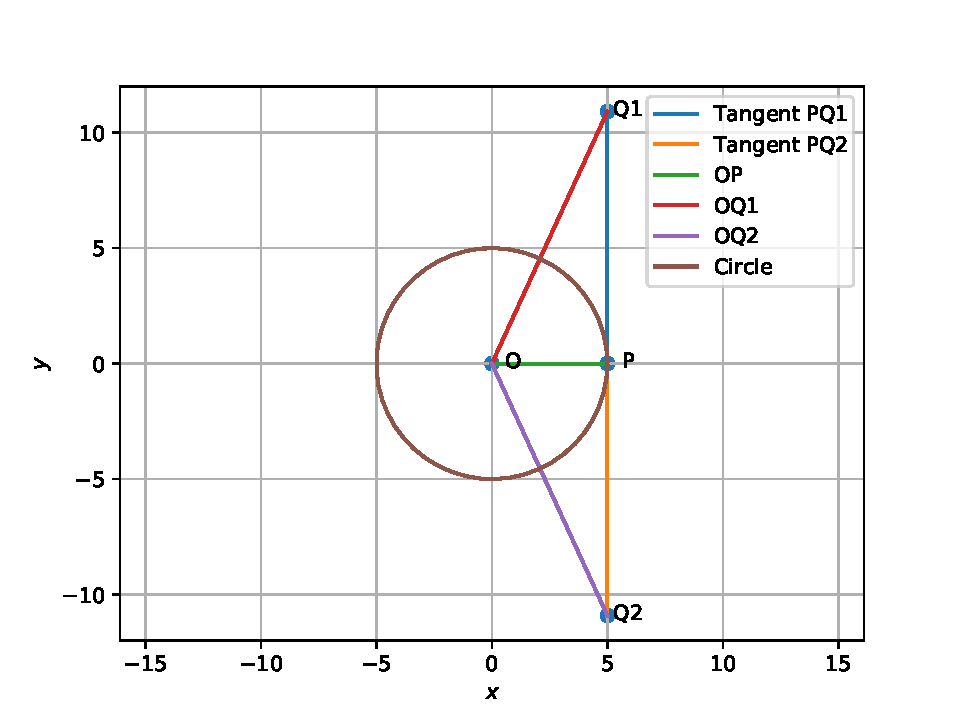
\includegraphics[width=\columnwidth]{figs/fig2.pdf}
\end{center}
\caption{}
\label{fig:Fig1}
\end{figure}
\end{enumerate}
\end{document}
